\section{Data Used}
\subsection{Initial Data}
%The initial architecture has been developed using a data package from LANL for a two-crack system. Data for 250 time steps was provided, with failure occurring at step 52. While useful for testing purposes, this mesh was much coarser than those of the true systems. Hence, for training the network, we used more representative systems of standard HOSS output.

Our preliminary investigation was localized to one LAMMPS simulation run. The data used contained information on bonds, atoms and rings, under the fully periodic condition.

\subsection{Training Data}
At the moment, data from one fully periodic simulation is used to train the base case model presented below.  Ultimately, we plan to generalize across different numbers of simulation to create a more sophisticated model and improve predicting accuracy. 

The features we use include cell volume, number of bonds and maximum ring size at initial time step. The label is the dummy indicator of whether or not a certain atom has ever been part of a 20-sized ring during the whole timesteps.


\section{Results}
In this section, we presents the preliminary results we obtained from base case toy models, which are Logistic Regression and Support Vector Machine with imbalanced class.

\subsection{Logistic Regression}
Logistic Regression is a static model that we use to predict the labels with probabilities of the underlying classes. However, due to imbalanced class, the model ignores the false negatives and predicts all the labels to be negative to obtain a high accuracy. 

\subsection{SVM with imbalanced class}
To tackle the problem of imbalanced class, we also implemented a Support Vector Machine model with a penalty,$c=1$, on the imbalanced classes. The model obtains an accuracy of 66\% and an area under the AUROC curve of 0.58.



\iffalse
\subsection{Crack Identification}
In converting HOSS FDEM output to graph form, recall that we follow two rules to preserve the integrity of the fracture network:
\begin{itemize}
	\item Edge crack identification must remain fixed over time.
 	\item Crack identity must be preserved through coalescence.
\end{itemize} 
By preserving the identification of each crack through both time and coalescence, we provide the necessary index for identification and tracking of each crack across all time steps, as well as correct attribution of feature metrics to the appropriate locations.
          
\subsection{Graph Data Matrices}
In order to set up the Graph Convolutional Neural Network architecture, we need to define the metrics used in the Adjacency and Feature matrices.\\
Distance Metrics:
        \begin{itemize}
        \item Coalescence (binary)
        \item Tip Intersect Distance  
        \item Shortest Euclidean Distance
        \item Minimum Damage Path
        \end{itemize}       
Features:
    \begin{itemize}
	\item Maximal horizontal projected crack tip Euclidean length
	\item Maximal vertical projected crack tip Euclidean length 
	\item Crack extreme tip Euclidean length
    \item Maximal Crack path Euclidean length between two tips
    \item Total path length including all crack tips
    \item Total crack damage
    \item Max tip stress
    \item Mean tip stress
	\end{itemize}
    
Functions were created to calculate and extract this data from HOSS simulation data to create graph data matrices for each HOSS time step.  

\section{R-GCN Setup}
The second milestone is to construct a working algorithm and model from the graph representation to predict the behavior of the fracture network over time. We accomplish this by using the Keras library for Python as a basis for building our RNN \cite{chollet2015keras}. The model simultaneously outputs predictions for both the features and each distance metric while following precisely the architecture presented in section 3.4. The implementation of the graph convolutional layer is taken from \cite{kipf2016semi}.

\section{Results}

As mentioned, our preliminary results come from training on three twenty-crack systems. In order to augment training data and increase the generalization ability of the network, we randomly take slices of 25 time steps. This allows for the network to learn from varying starting points and works to prevent overfitting. Also, the features are normalized across feature type before training using a normalizing matrix. Given that some features, such as total crack damage, can become large near the end of the system this serves to condense values to a far smaller range and enable better learning. Ultimately, the feature predictions can be transformed back to their original scale through the same normalizing matrix from the training data.

Our goal is for our network to be able to generalize, to predict systems on which it has not been trained. However, for these initial tests, we perform the more simple task of predicting the evolution of one of the three crack systems from time step 0 to the final time step. As described in the methods section, there will first be a prediction for time step 1 given input at time step 0, then for time step 2 given input at time steps 0 and predicted output from time step 1 and so on. This will test the general ability of the architecture to learn and find patterns.

\begin{figure}[!htb]
\centering
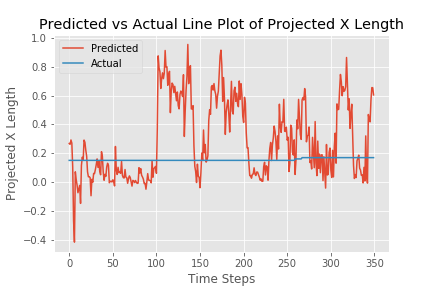
\includegraphics[width=0.8\textwidth]{images/Projected_X_Length_compare_transformed}
\caption{Plot comparing the predicted values against true values for projected $x$ length of crack 19.}
\label{fig:proj_y}
\end{figure}

\begin{figure}[!htb]
\centering
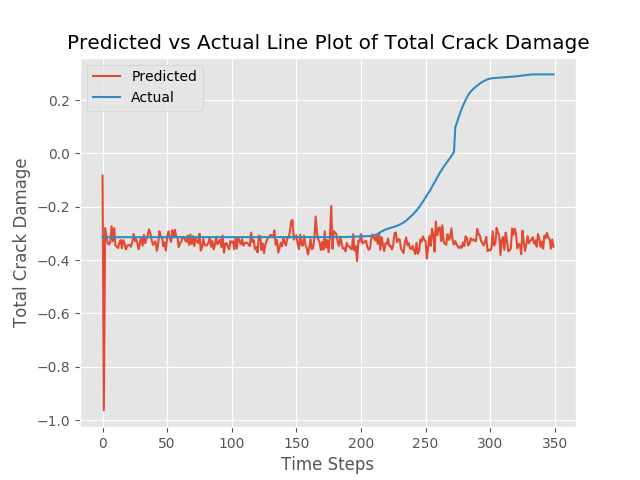
\includegraphics[width=0.8\textwidth]{images/Total_Crack_Damage_compare}
\caption{Plot comparing the normalized predicted values against the normalized true values for total crack damage in crack 4.}
\label{fig:tot_dam}
\end{figure}

In figures \ref{fig:proj_y} and \ref{fig:tot_dam}, selected results for feature prediction are presented. In figure \ref{fig:proj_y},we plot the projected $x$ length vs.\ time, for a simulated system with total size of 3 in the $x$ direction and 2 and in the $y$ direction.
%The spatial scale of the material in this simulation run is 3 by 2( Total X length 3, Y length 2).
The actual projected $x$ length does not change until time step 200.  Many of the features in a given simulation are essentially constant, and thus in our limited training, the model has overfit to these examples. This is illustrated in figure \ref{fig:tot_dam}, where the damage changes near the end of the simulation, yet our network is unable to predict the change.

As the output from HOSS is not deterministic, the comparison between distributions of crack features is more meaningful than feature comparisons on specific cracks. In figure \ref{fig:mean_proj_x_length}, we plot our prediction for the mean projected $x$ length of all cracks, along with the actual mean projected $x$ length. The band represents plus and minus one standard deviation of the crack features. As we can see, the mean and variance in our prediction is tracking the actual when the cracks start growing quickly around time step 220.

Ultimately, these preliminary results showed us that the network has the ability to learn. It does not predict each feature perfectly, yet it does give meaningful predictions for distributions over all cracks in the system. These results leave us optimistic for future results given additional network refinement and more substantial training.

\begin{figure}[!htb]
\centering
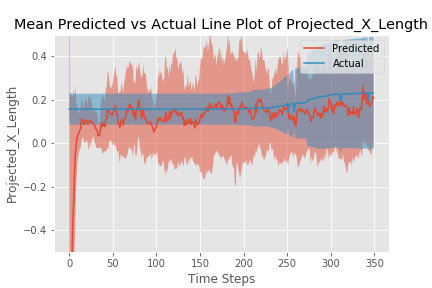
\includegraphics[width=0.8\textwidth]{images/Projected_X_Length_mean_variance_compare_ylim_test}
\caption{Plot comparing the mean predicted values against mean true values for projected $x$ length of all cracks. Shaded bands show one standard deviation above and below mean.}
\label{fig:mean_proj_x_length}
\end{figure}

\section{Remaining Milestones}
The two remaining milestones serve as goalposts for the second half of the CGU Math Clinic year:
\begin{itemize}
\item Determine the importance of different crack features for the prediction of the evolution of the fracture network.
\item Refine and add complexity to the network (i.e.,\ additional convolutional filters, layered graph convolution, compare effectiveness of spectral clustering graph convolutions versus standard graph convolutions).
\end{itemize}



\section{Deliverable Status}
\begin{enumerate}
\item Keras implementation of proposed architecture, coded in Python.
	\begin{itemize}
		\item In progress.
	\end{itemize} 
\item Full documentation of code in iPython Notebook.
	\begin{itemize}
		\item In progress. On track to be finalized along with final code.
	\end{itemize} 
\item Midterm presentation.
	\begin{itemize}
		\item Complete, November 14, 2017.
	\end{itemize} 
\item Mid-year report.
	\begin{itemize}
		\item Complete, December 18, 2017.
	\end{itemize} 
\item Journal article on the dynamic prediction of the fracture of brittle material using deep learning, submitted to peer-reviewed journal.
	\begin{itemize}
		\item Forthcoming, Spring 2018.
	\end{itemize} 
\item Final presentation.
	\begin{itemize}
		\item Forthcoming, Spring 2018.
	\end{itemize} 
\item Final report.
	\begin{itemize}
		\item Forthcoming, Spring 2018.
	\end{itemize} 
\end{enumerate}
\fi